\chapter{Introdução}
\label{cap:introducao}

Nesta seção, são apresentados o contexto da pesquisa, a motivação, a metodologia da
pesquisa e as discussões e soluções que fundamentam este trabalho.

\section{Contexto da Pesquisa}
\label{sec:contexto}

Nos últimos anos, a relevância dos fatores ambientais, sociais e de governança (\gls{ESG}) têm
crescido significativamente no contexto empresarial e financeiro. A sigla ESG, utilizada
oficialmente pela primeira vez em um relatório da ONU, intitulado ``Who Cares Wins'' em 2004
\cite{onu2004}, refere-se a critérios que medem a sustentabilidade e o impacto ético de um
investimento em uma empresa. Desde então, os Princípios para Investimentos Responsáveis
(\gls{PRI}) da ONU, estabelecidos em 2006 \cite{onu2006}, reforçaram a importância dos critérios
ESG como princípios financeiros, formando a base da estrutura ESG que conhecemos hoje.

A pandemia de COVID-19 intensificou a atenção global aos temas ESG, especialmente em
relação às mudanças climáticas, proteção ambiental e saúde pública. A importância dos
investimentos a longo prazo, que consideram os riscos e oportunidades associados aos critérios
ESG, tornou-se mais evidente durante este período. As avaliações de processos econômicos
corporativos com base em ESG passaram a fornecer uma visão mais ampla, abrangendo tanto
posições regionais quanto globais.

Diversos estudos têm explorado a relação entre os conceitos de ESG e os investidores,
utilizando dados específicos de países ou focando em mercados financeiros específicos. Por
exemplo, alguns trabalhos analisaram como os dados de linguagem natural relacionados a ESG
impactam os mercados financeiros, enquanto outros examinaram os relatórios de responsabilidade
social corporativa (\gls{CSR}) para entender as concepções ESG. No entanto, esses estudos
frequentemente utilizam dados limitados ou não abrangem uma análise ampla, deixando lacunas no
entendimento sobre a utilização dos critérios ESG.

Neste contexto, a análise de sentimentos aplicada a dados relacionados a ESG emerge como
uma ferramenta para capturar as percepções públicas e acadêmicas. A análise de sentimentos, uma
subárea do processamento de linguagem natural (\gls{NLP}), permite a identificação de opiniões e
emoções expressas em textos, como notícias e publicações acadêmicas. Esta pesquisa busca auxiliar
na solução de um problema prático do mundo real utilizando a metodologia denominada Design
Science \cite{wieringa2014} para sua condução. Para isto seguiu-se uma estrutura lógica para
resolução do problema.

\section{Motivação}
\label{sec:motivacao}

Plataformas de exploração urbana e turística estão redefinindo a maneira como as pessoas se
conectam com os lugares, seu patrimônio e as narrativas locais. Ao permitir que os usuários
expressem suas impressões e vivências, abre-se uma nova janela para compreender a percepção e a
construção da identidade territorial. Neste contexto, a análise de sentimento emerge como uma
abordagem central para decifrar as nuances dessas interações e entender profundamente o que os
usuários sentem.

A ferramenta foco deste estudo, ao ser utilizada para explorar roteiros culturais ou interagir
com narrativas urbanas, não apenas guia o usuário, mas também se torna um canal para capturar
suas ricas experiências subjetivas. A aplicação da análise de sentimento sobre esses registros
permite identificar padrões emocionais e avaliar como as características de um lugar e as narrativas
associadas a ele ressoam com o público. O desenvolvimento e aprimoramento de uma solução
tecnológica com este propósito seguem uma abordagem metodológica estruturada, como a Design
Science, que orienta a criação de artefatos para solucionar problemas práticos e investigar
fenômenos reais. Entender, por exemplo, como o fato de ter nascido e/ou crescido em determinada
comunidade influenciou características culturais, sociais e aptidões políticas de um indivíduo é
crucial para definição de políticas públicas voltadas para educação e cultura daquele lugar, visando
preservar heranças passadas ou mesmo melhorar aspectos negativos identificados.

A análise sistemática das percepções e dos sentimentos dos usuários, capturados e
interpretados através desta plataforma, pode oferecer contribuições valiosas. Essas contribuições
podem direcionar também o aprimoramento de experiências turísticas e culturais, tornando-as mais
envolventes e significativas. Podem também informar como as pessoas estão percebendo e
construindo sua identidade com os espaços mediados pela ferramenta, fornecendo subsídios para
que esta se torne ainda mais eficaz em promover uma relação positiva com o entorno. A
compreensão profunda das reações emocionais, obtida via análise de sentimento, possibilita o
desenvolvimento de intervenções e recomendações mais personalizadas e eficazes através de
ferramentas de software, fortalecendo a conexão emocional e o senso de identidade dos usuários
com os lugares que exploram. Portanto, esta pesquisa se dedica a investigar como a análise de
sentimento aplicada aos dados gerados no Gnomon, uma plataforma digital interativa de exploração
urbana e turística, pode revelar e medir a percepção e a identidade de lugar formadas pelos seus
usuários.

\section{Metodologia da Pesquisa}
\label{sec:metodologia-pesquisa}

Para este trabalho seguiu-se uma estrutura lógica para resolução do problema. A seguir, as
questões de pesquisas que orientam este trabalho.

\subsection{Questões de Pesquisa}
\label{subsec:questoes-pesquisa}

As questões de pesquisa deste estudo empregam a abordagem Design Science para ajudar na
identificação dos problemas. Uma investigação guiada pelo Design Science adota uma metodologia
baseada na resolução de problemas \cite{wieringa2009}.

Em um cenário onde a responsabilidade social e a sustentabilidade se tornam cada vez mais
cruciais para a reputação e o sucesso das organizações, utilizar a análise de sentimento para melhorar
o desempenho ESG de organizações públicas é uma abordagem válida. Primeiramente, a análise de
sentimento permite que tenhamos a percepção do público sobre suas práticas ESG. Isso possibilita
uma resposta rápida a críticas e preocupações, demonstrando transparência. Além disso, com a
análise de grandes volumes de dados provenientes de redes sociais, notícias e outras fontes, é
possível identificar tendências e potenciais problemas antes que se tornem crises de reputação,
essencial para a gestão proativa das práticas ESG. Entender o sentimento do público também ajuda as
organizações a adaptar suas estratégias de comunicação, tornando-as mais eficazes. Mensagens que
ressoam com os valores e preocupações da sociedade podem aumentar o engajamento e o apoio às
iniciativas ESG. Ademais, a análise de sentimento pode fornecer informações sobre áreas onde as
práticas ESG podem ser melhoradas, permitindo que as organizações implementem mudanças
direcionadas e monitorem o impacto dessas melhorias ao longo do tempo. Então a questão geral de
pesquisa a ser tratada neste trabalho compreende:

\begin{citacao}
Como melhor identificar a percepção das pessoas sobre as práticas ESG e sua identidade de lugar?
\end{citacao}

Do ponto de vista organizacional, essa questão de pesquisa pode ser decomposta em outras
questões elementares. Segundo a Design Science, esta questão geral de pesquisa pode ser
categorizada em Questões Conceituais (QC), Questões Técnicas (QT) e Questões Práticas (QP).
Dessa forma, a Questão de Pesquisa enunciada acima pode ser decomposta nas seguintes questões de
pesquisa apresentadas a seguir:

\begin{alineas}
    \item \textbf{QC 1}: O que são Indicadores ESG?
    \begin{alineas}
        \item \textit{Explicação}: Essa questão busca identificar quais aspectos do ESG são mais relevantes e como eles podem ser representados em dados textuais para a análise de sentimento.
        \item \textit{Motivação}: Compreender os indicadores ESG e como eles funcionam.
    \end{alineas}
    \item \textbf{QT 2}: Como por meio de algoritmos de análise de sentimento podemos avaliar aspectos de ESG?
    \begin{alineas}
        \item \textit{Explicação}: Esta questão examina quais algoritmos de processamento de linguagem natural são mais eficazes para a análise de ESG.
        \item \textit{Motivação}: Identificar os algoritmos mais adequados pode melhorar a precisão e a relevância dos resultados obtidos.
    \end{alineas}
    \item \textbf{QP 3}: Como esses resultados podem ser utilizados para melhorar as práticas de ESG?
    \begin{alineas}
        \item \textit{Explicação}: Investigar formas práticas de aplicação dos valores obtidos pela análise de sentimento para promover melhorias nas práticas de ESG.
        \item \textit{Derivadas}: Quais são os principais desafios na implementação de melhorias baseadas em análise de sentimento?
    \end{alineas}
\end{alineas}

Em Design Science, a estruturação do conjunto de problemas de pesquisa é realizada através
da decomposição de uma questão geral de pesquisa em questões conceituais, técnicas e práticas. A
construção do conjunto de soluções ocorre pela composição das soluções apresentadas para essas
questões.

\subsection{Métodos de Pesquisa}
\label{subsec:metodos-pesquisa}

Para alcançar os objetivos pretendidos a pesquisa seguiu um conjunto de fases de acordo com
o Design Science \cite{wieringa2014}. O espaço-problema define a questão geral de pesquisa (QGP)
que foi decomposta em questões conceituais (QC), técnicas (QT) e práticas (QP). O espaço-solução
define as contribuições, composta pelos artefatos que respondem o conjunto de questões, conforme
ilustrado na Figura \ref{fig:metodologia-pesquisa}.

\begin{figure}[h]
    \centering
    \caption{Metodologia de Pesquisa}
    \label{fig:metodologia-pesquisa}
    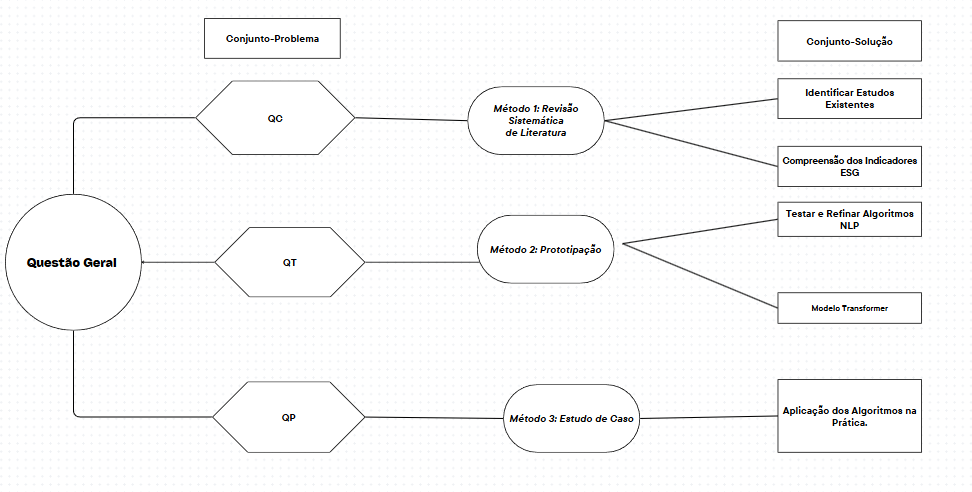
\includegraphics[width=0.85\textwidth]{figuras/metodologia-pesquisa}
    \legend{Fonte: Autoria Própria (2024).}
\end{figure}

Para responder às questões de pesquisa relacionadas ao uso de algoritmos de análise de
sentimento, com o intuito de melhorar o desempenho ESG (\textit{Environmental, Social, and Governance}),
serão adotados os seguintes métodos de pesquisa:

\begin{alineas}
    \item \textbf{Revisão Sistemática da Literatura (\gls{RSL})}: A RSL será utilizada para identificar e analisar estudos existentes sobre a aplicação de algoritmos de análise de sentimento em ESG. Este método permitirá uma compreensão abrangente dos principais indicadores ESG que podem ser extraídos de textos.
    \begin{alineas}
        \item \textit{Definição do Protocolo de RSL}: Estabelecer critérios de inclusão e exclusão, bases de dados a serem utilizadas e estratégias de busca.
        \item \textit{Coleta de Dados}: Realizar buscas em bases de dados acadêmicas como IEEE Xplore, ACM e Google Scholar.
        \item \textit{Análise e Sumarização}: Revisar e sintetizar os resultados dos estudos relevantes encontrados.
    \end{alineas}
    \item \textbf{Prototipação e Desenvolvimento}: A prototipação será utilizada para testar algoritmos de análise de sentimento adaptados ao contexto ESG. Este processo envolverá várias etapas de desenvolvimento, teste e refinamento.
    \begin{alineas}
        \item \textit{Seleção de Algoritmos}: Identificar algoritmos de NLP adequados, como modelos de Transformer (Modelo de rede Neural).
        \item \textit{Treinamento e Validação}: Treinar os algoritmos utilizando conjuntos de dados textuais relevantes (mídias sociais, relatórios financeiros, notícias) e validar sua eficácia com métricas como precisão, \textit{Recall} e F1-\textit{score}.
        \item \textit{Ajustes e Melhorias}: Refinar os algoritmos com base nos resultados.
    \end{alineas}
    \item \textbf{Estudo de Caso}: Aplicar os algoritmos desenvolvidos em um estudo de caso real para validar sua eficácia prática. Este estudo envolverá a utilização dos dados do Gnomon em situações reais.
    \begin{alineas}
        \item \textit{Seleção do Caso}: Definir um ou mais cenários de uso da ferramenta de exploração urbana e turística que permitam a coleta de dados relevantes para a análise de percepção e identidade de lugar.
        \item \textit{Coleta de Dados}: Obter dados gerados a partir da interação dos usuários com a ferramenta, como comentários, avaliações, e outros registros textuais que expressem suas percepções e sentimentos sobre os lugares explorados.
        \item \textit{Aplicação dos Algoritmos}: Aplicar os algoritmos de análise de sentimento para identificar e analisar as percepções dos usuários sobre os lugares e a formação de identidade de lugar, a partir dos dados coletados pela ferramenta.
        \item \textit{Avaliação dos Resultados}: Analisar os resultados gerados sobre a percepção e identidade de lugar, e avaliar a eficácia dos algoritmos e da ferramenta em capturar e interpretar esses aspectos, utilizando os resultados para refinar os algoritmos e métodos.
    \end{alineas}
\end{alineas}

\section{Discussões e Soluções}
\label{sec:discussoes-solucoes}

A revisão da literatura e a aplicação da ferramenta digital Gnomon em um estudo de caso
permitirão identificar aspectos da percepção de lugar e identidade territorial a partir de textos de
usuários, utilizando análise de sentimento. A eficácia de Modelos de Linguagem de Grande Porte
(\gls{LLM}s), como a \gls{API} Gemini, será avaliada para esta tarefa, com o suporte de estudos da
\gls{RSL} que demonstram o potencial de modelos NLP avançados como \gls{BERT} e \gls{RoBERTa}
para análises textuais detalhadas \cite{schimanski2024, gupta2024}.

A análise de sentimento buscará compreender profundamente como os usuários percebem os
lugares e expressam sua identidade ao usar o Gnomon. Esses resultados informarão o aprimoramento
da plataforma para enriquecer a experiência do usuário e sua conexão com o patrimônio e ambientes
explorados. No âmbito da Design Science, os resultados da análise de sentimento não apenas
responderão à questão de pesquisa sobre a identificação da percepção e identidade de lugar, mas
também oferecerão orientações práticas para o aprimoramento contínuo. O objetivo é fomentar o
desenvolvimento de experiências digitais mais significativas, personalizadas e que efetivamente
valorizem a relação humano-lugar.
